\chapter{Experiment}\label{chap:experiment}

Three sets of experiments have been conducted. A migration tweet detection(MTD) was executed at the beginning of the project, exploring the performance of the three classifier. A sentiment detection(SD) model is built using annotated data, performance metric are computed. Tweets which are classified as migration tweets are passed to sentiment detection model to detect its sentiment.

\section{Evaluation Measures}

In order to evaluate the performance of the classifier, all three in the case of migration detection, sentiment classification and in the end detecting the sentiment of migration classified tweets we adopt the common standards in the respective fields. All assessment metrics described in this section are shown in Section \ref{metricsofclassification}

\subsection{Migration Detection Scoring}
In MTD each tweet is classified as being either in a ``yes" or ``no" classes, thus MTD is a binary classification problem. It is normal to report the precision, recall, and F1 scores. Additionally, it is common to report the accuracy of predicted clases. We report these metrics in all of our MTD experiments.



\subsection{Sentiment Detection Scoring}
Just like the MTD, SD is also binary classifier. Here, each tweet is classified as either ``positive" or ``negative". We report precision, recall, F1 scores and the accuracy of the classifier model.

\subsection{Detecting the sentiment of migration tweets - Scoring}
Evaluating this experiment is different from previous two steps. Here the Tweets which classified only ``yes" class from MTD, are passed to ST to classify them as ``positive" or ``negative" classes.  The migration tweets from MTD are also annotated with their respective sentiment labels in tweet annotation step. This step to annotate the sentiment of migration tweets is considered as the ground truth, and we report precision, recall, F1 scores and the accuracy of the classifier model comparing with the ground truth value.




\section{Migration detection experiment} \label{migration_detection_experiment}
This section describes the steps which were conducted while building migration detection model. A typical text classification, tries to extract a featureset from the text using some feature extraction methods, which are discussed in \ref{backgroundworkFeatureEngi}. In this research, in order to increase the accuracy of the classifier, additional features are added to featureset, based on the presence of the specific terms which are related to ``Human migration". Then the model is evaluated using the metrics as discussed in \ref{metricsofclassification}.    

\subsection{Experiment Description}
To implement the Migration detection the following steps were undertaken:

\subsubsection{Data-set collection}
The twitter archives \footnote{\url{https://archive.org/}} were considered to collect the data for the migration detection model. The archives are collection of tweets for one month. A python script would unzip the archive file, parse all the files into JSON format, and searches each JSON object for the presence of the listed hahtags (\#refugee, \#wall, \#Syria, \#syrianrefugee,
\#mexicanwall, \#trumpwall, \#immigrants). If present, the text of the tweet and the user's description is saved in to csv file.  A total of 1275 tweets were collected from data archive(100GB).



\subsubsection{Prepossessing} \label{sssec:preprocessing}

Data prepossessing is fundamental step to all data science and
Natural Language Processing Tasks. The prepossessing steps in
our project is common to both migration detection and sentiment detection models the models. After retrieving the JSON, the prepossessing script performs the following steps:
\begin{enumerate}
    \item Take only lines with "English" language Tweets.
    \item Sort the tweets, Check similarity between consecutive tweets , if similarity is greater than 80\%, remove the duplicate tweets.
    \item Search for the full\_text of the tweet (In cases of re-tweets or too big tweets, additional attributes are added to the tweet.
    \item Deleting all non-alphanumeric characters.
\end{enumerate}
The scripts are mainly implemented using the regular expression. The prepossessed tweets are manual annotated with label ``yes" and ``no". After this step the data is clean and is passed to feature engineering step. Distribution of obtained tweets are show in the figure \ref{fig:graphDistmigration}.

\begin{figure}
	\centering
	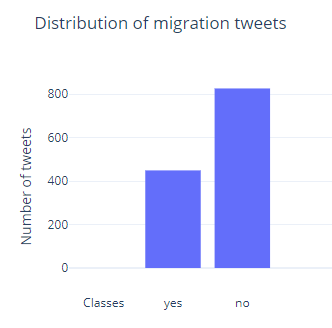
\includegraphics[width=10cm\linewidth,height=10cm]{thesis_template/images/distofmigration_tweetsundefined.png}
	\caption{Distribution of the migration tweets}
	\label{fig:graphDistmigration}
\end{figure}


\subsubsection{Feature engineering }
Feature Engineering starts from an initial set of measured data and
build derived values (features) which is intended to be informative. In this project, Count vectorizer is used to extract feature from the text of the tweet. Along with that Migration index(MI) and migration percentage(MP) is calculated, section \ref{featureengineering} discusses the process of computing MI and MP. Count vector is a sparse matrix, this feature is combined with MP and MI feature using feature union technique, section \ref{backgroundworkFeatureEngi} discusses the technique of feature union.  

\subsubsection{Classification and Metrics}
The classifier is treated as a binary classifier, with the labels ``yes" and ``no". The label ``yes" represents the  migration tweet and the label ``no" represents the tweet is not a migration tweet. The dataset is split into train(75\%) and test sets(25\%). 

Three classifier are used in this project, naive Bayes, Logistic regression, decision trees. Performance metric of all the three classifier is given in table \ref{tab:Migration_metric}

\begin{itemize}
    \item Naive Bayes
    
    The confusion matrix of migration detection from the naive Bayes model is show in the table \ref{tab:confusionmatrix_migrationtweets_nb}

\begin{table}[]
\centering
\begin{tabular}{lllll}
\cline{1-3}
\multicolumn{1}{|l|}{}   & \multicolumn{1}{l|}{predicted\_YES} & \multicolumn{1}{l|}{predicted\_NO}  &  &  \\ \cline{1-3}
\multicolumn{1}{|l|}{YES} & \multicolumn{1}{l|}{78}  & \multicolumn{1}{l|}{25} &  &  \\ \cline{1-3}
\multicolumn{1}{|l|}{NO}   & \multicolumn{1}{l|}{32}  & \multicolumn{1}{l|}{184}  &  &  \\ \cline{1-3}
                            &                           &                           &  & 
\end{tabular}
\caption{Naive Bayes: Confusion matrix for migration model}
\label{tab:confusionmatrix_migrationtweets_nb}
\end{table}

    
    \item Logistic regression
    
    The confusion matrix of migration detection model using the logistic regression algorithm is show in the table \ref{tab:confusionmatrix_migrationtweets} .

\begin{table}[]
\centering
\begin{tabular}{lllll}
\cline{1-3}
\multicolumn{1}{|l|}{}   & \multicolumn{1}{l|}{predicted\_YES} & \multicolumn{1}{l|}{predicted\_NO}  &  &  \\ \cline{1-3}
\multicolumn{1}{|l|}{YES} & \multicolumn{1}{l|}{87}  & \multicolumn{1}{l|}{16} &  &  \\ \cline{1-3}
\multicolumn{1}{|l|}{NO}   & \multicolumn{1}{l|}{4}  & \multicolumn{1}{l|}{212}  &  &  \\ \cline{1-3}
                            &                           &                           &  & 
\end{tabular}
\caption{Logistic regression: Confusion matrix for migration model}
\label{tab:confusionmatrix_migrationtweets}
\end{table}

    \item Decision trees
    
    The confusion matrix of the migration detection model using decision trees algorithm can be found in the table.
 \ref{tab:confusionmatrix_migrationtweets_DT} 

\begin{table}[]
\centering
\begin{tabular}{lllll}
\cline{1-3}
\multicolumn{1}{|l|}{}   & \multicolumn{1}{l|}{predicted\_YES} & \multicolumn{1}{l|}{predicted\_NO}  &  &  \\ \cline{1-3}
\multicolumn{1}{|l|}{YES} & \multicolumn{1}{l|}{90}  & \multicolumn{1}{l|}{13} &  &  \\ \cline{1-3}
\multicolumn{1}{|l|}{NO}   & \multicolumn{1}{l|}{7}  & \multicolumn{1}{l|}{209}  &  &  \\ \cline{1-3}
                            &                           &                           &  & 
\end{tabular}
\caption{Decision trees: Confusion matrix for migration model}
\label{tab:confusionmatrix_migrationtweets_DT}
\end{table}
\end{itemize}

 The dataset is imbalanced with majority of samples in "no" class as shown in figure \ref{fig:graphDistmigration}. Which, explains why many samples are predicted as negative class from the confusion matrix [tables \ref{tab:confusionmatrix_migrationtweets_DT}, \ref{tab:confusionmatrix_migrationtweets_nb}, \ref{tab:confusionmatrix_migrationtweets}]  of all the classifier. Performance metrics of the three classifier is show in the table \ref{tab:Migration_metric}. In particular, the logistic regression and decision trees have nearly the same accuracy and F1 score. The performance of naive bayes compared to, other two classifier is low.

\begin{table}[]
\centering
\begin{tabular}{lllll}
\hline
\textbf{Classifier} & \textbf{Accuracy} & \textbf{Precision} & \textbf{Recall} & \textbf{F1-score} \\ \hline
Logistic regression & 0.937             & 0.956              & 0.844           & 0.896             \\ \hline
Naive Bayes         & 0.821             & 0.709              & 0.757           & 0.732             \\ \hline
Decision Trees     & 0.943             & 0.938              & 0.883           & 0.909             \\ \hline
\end{tabular}
\caption{Performance metric of all the classifier - Migration model}
\label{tab:Migration_metric}
\end{table}


\section{Sentiment detection model} \label{snetimentdetectionmodel}

This section describes the steps which were conducted while building sentiment detection
model. A data set from the Stanford Twitter Corpus \footnote{\url{http://help.sentiment140.com/for-students/}} was used for the sentiment detection model, which is annotated with positive and negative labels. Countvectorizer \cite{scikit-learn} library from scikit learn is used to convert the text into vectors. The vectors along the target labels are used to build a classifier. Distribution of the tweets is shown in the figure \ref{fig:graphDistsentiment} 
 




\subsection{Prepossessing}
A python script performs reads each line from the dataset and performs the following reprocessing steps:
\begin{enumerate}
    \item Take only lines with "English" language Tweets.
    \item Sort the tweets, Check similarity between consecutive tweets , if similarity is greater than 80\%, remove the duplicate tweets.
    \item Search for the full\_text of the tweet (In cases of re-tweets or too big tweets, additional attributes are added to the tweet.
    \item Deleting all non-alphanumeric characters.
\end{enumerate}
Regular expression was used to perform this actions, the cleaned data is passed to feature engineering step Distribution of obtained tweets are show in the figure \ref{fig:graphDistsentiment}


\begin{figure}
	\centering
	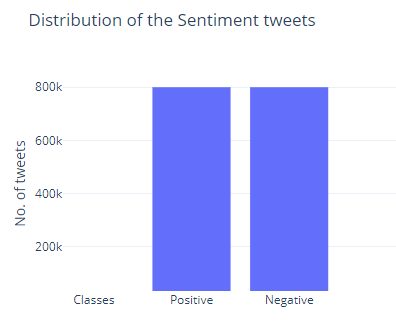
\includegraphics[width=12cm\linewidth,height=10cm]{thesis_template/images/distofsentiment_tweetsundefined.png}
	\caption{Distribution of the sentiment tweets}
	\label{fig:graphDistsentiment}
\end{figure}



\subsection{Classification and Metrics}
This classification is treated as a binary classifier with " positive " and " negative " labels. The " positive " label is the positive sentiment of the tweet and the " negative " label is the negative snetiment of the tweet. The dataset is split into train(98\%), test sets(1\%) and validation set(1\%). The performance of the three classifier is compared.

\begin{itemize}
    \item  Naive Bayes
    
    The confusion matrix of sentiment detection from the naive Bayes model is show in the table \ref{tab:confusionmatrix_sentimenttweets_NB}
    
    \begin{table}[]
\centering
\begin{tabular}{lllll}
\cline{1-3}
\multicolumn{1}{|l|}{}   & \multicolumn{1}{l|}{predicted\_POS} & \multicolumn{1}{l|}{predicted\_NEG}  &  &  \\ \cline{1-3}
\multicolumn{1}{|l|}{POS} & \multicolumn{1}{l|}{6338}  & \multicolumn{1}{l|}{1656} &  &  \\ \cline{1-3}
\multicolumn{1}{|l|}{NEG}   & \multicolumn{1}{l|}{1494}  & \multicolumn{1}{l|}{6472}  &  &  \\ \cline{1-3}
                            &                           &                           &  & 
\end{tabular}
\caption{Naive Bayes: Confusion matrix for sentiment model}
\label{tab:confusionmatrix_sentimenttweets_NB}
\end{table}

\item  Logistic Regression
    
    The confusion matrix of sentiment detection from the logistic regression model is show in the table \ref{tab:confusionmatrix_sentimenttweets_LR}
    
    \begin{table}[]
\centering
\begin{tabular}{lllll}
\cline{1-3}
\multicolumn{1}{|l|}{}   & \multicolumn{1}{l|}{predicted\_POS} & \multicolumn{1}{l|}{predicted\_NEG}  &  &  \\ \cline{1-3}
\multicolumn{1}{|l|}{POS} & \multicolumn{1}{l|}{6720}  & \multicolumn{1}{l|}{1274} &  &  \\ \cline{1-3}
\multicolumn{1}{|l|}{NEG}   & \multicolumn{1}{l|}{1489}  & \multicolumn{1}{l|}{6477}  &  &  \\ \cline{1-3}
                            &                           &                           &  & 
\end{tabular}
\caption{Logistic regression: Confusion matrix for sentiment model}
\label{tab:confusionmatrix_sentimenttweets_LR}
\end{table}

\item  Decision Trees
    
    The confusion matrix of sentiment detection from the Decision trees model is show in the table \ref{tab:confusionmatrix_sentimenttweets_DT}
    
    \begin{table}[]
\centering
\begin{tabular}{lllll}
\cline{1-3}
\multicolumn{1}{|l|}{}   & \multicolumn{1}{l|}{predicted\_POS} & \multicolumn{1}{l|}{predicted\_NEG}  &  &  \\ \cline{1-3}
\multicolumn{1}{|l|}{POS} & \multicolumn{1}{l|}{5923}  & \multicolumn{1}{l|}{2130} &  &  \\ \cline{1-3}
\multicolumn{1}{|l|}{NEG}   & \multicolumn{1}{l|}{2031}  & \multicolumn{1}{l|}{5876}  &  &  \\ \cline{1-3}
                            &                           &                           &  & 
\end{tabular}
\caption{Decision trees: Confusion matrix for sentiment model}
\label{tab:confusionmatrix_sentimenttweets_DT}
\end{table}
     
\end{itemize}


 The dataset is balanced with equal number of samples on both the classes as shown in figure \ref{fig:graphDistsentiment}. Which, explains why many samples are predicted as negative class from the confusion matrix [tables \ref{tab:confusionmatrix_migrationtweets_DT}, \ref{tab:confusionmatrix_migrationtweets_nb}, \ref{tab:confusionmatrix_migrationtweets}]  of all the classifier. Performance metrics of the three classifier is show in the table \ref{tab:Migration_metric}. In particular, the logistic regression and decision trees have nearly the same accuracy and F1 score. The performance of naive Bayes compared to, other two classifier is low.

\begin{table}[]
\centering
\begin{tabular}{lllll}
\hline
\textbf{Classifier} & \textbf{Accuracy} & \textbf{Precision} & \textbf{Recall} & \textbf{F1-score} \\ \hline
Logistic regression & 82.69             & 0.83              & 0.83           & 0.83             \\ \hline
Naive Bayes         & 80.38             & 0.80              & 0.80           & 80             \\ \hline
Decision Trees     & 73.93             &  0.74              &  0.74           &  0.74             \\ \hline
\end{tabular}
\caption{Performance metric of all the classifier - Migration model}
\label{tab:sentiment_metric}
\end{table}




\section{Sentiment detection of migration classified tweets - experiment}

This is the important step in this research, in this step tweets classified as migration tweets from the migration detection model are passed to the sentiment detection model.

\subsection{Experiment Description}

A python script reads the output of the migration detection model and filters only migration tweets. The migration tweets are also annotated with their respective sentiment labels in tweet annotation step. This step to annotate the sentiment of migration tweets is considered as the ground truth. The sentiment model would predict the sentiment of these migration tweets. Then the performance of the sentiment detection is calculated by comparing the ground truth and the predicted values. The number of tweets which are classified as the migration tweets is 449 tweets, and the distribution of the annotated sentiment labels is shown in the figure \ref{fig:sent_migration_distribution}. The performance metric of detecting the sentiment of these tweets are shown in table \ref{tab:sentiment_of_Migration_metric}

 

\begin{figure}
	\centering
	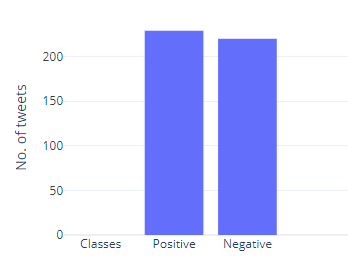
\includegraphics[width=12cm\linewidth,height=10cm]{thesis_template/images/sentiment_of_migration_tweets.png}
	\caption{ The distribution of "sentiment labels" for the classified migration tweets.}
	\label{fig:sent_migration_distribution}
\end{figure}


\begin{itemize}
    \item  Naive Bayes
    
    The confusion matrix of sentiment detection from the naive Bayes model is show in the table \ref{tab:confusionmatrix_sentimentmigrationtweets_NB}
    
    \begin{table}[]
\centering
\begin{tabular}{lllll}
\cline{1-3}
\multicolumn{1}{|l|}{}   & \multicolumn{1}{l|}{predicted\_POS} & \multicolumn{1}{l|}{predicted\_NEG}  &  &  \\ \cline{1-3}
\multicolumn{1}{|l|}{POS} & \multicolumn{1}{l|}{197}  & \multicolumn{1}{l|}{32} &  &  \\ \cline{1-3}
\multicolumn{1}{|l|}{NEG}   & \multicolumn{1}{l|}{164}  & \multicolumn{1}{l|}{56}  &  &  \\ \cline{1-3}
                            &                           &                           &  & 
\end{tabular}
\caption{Naive Bayes: Confusion matrix}
\label{tab:confusionmatrix_sentimentmigrationtweets_NB}
\end{table}

\item  Logistic Regression
    
    The confusion matrix of sentiment detection from the logistic regression model is show in the table \ref{tab:confusionmatrix_sentimentmigrationtweets_LR}
    
    \begin{table}[]
\centering
\begin{tabular}{lllll}
\cline{1-3}
\multicolumn{1}{|l|}{}   & \multicolumn{1}{l|}{predicted\_POS} & \multicolumn{1}{l|}{predicted\_NEG}  &  &  \\ \cline{1-3}
\multicolumn{1}{|l|}{POS} & \multicolumn{1}{l|}{184}  & \multicolumn{1}{l|}{45} &  &  \\ \cline{1-3}
\multicolumn{1}{|l|}{NEG}   & \multicolumn{1}{l|}{140}  & \multicolumn{1}{l|}{80}  &  &  \\ \cline{1-3}
                            &                           &                           &  & 
\end{tabular}
\caption{Logistic regression: Confusion matrix}
\label{tab:confusionmatrix_sentimentmigrationtweets_LR}
\end{table}

\item  Decision Trees
    
    The confusion matrix of sentiment detection from the Decision trees model is show in the table \ref{tab:confusionmatrix_sentimentmigrationtweets_DT}
    
    \begin{table}[]
\centering
\begin{tabular}{lllll}
\cline{1-3}
\multicolumn{1}{|l|}{}   & \multicolumn{1}{l|}{predicted\_POS} & \multicolumn{1}{l|}{predicted\_NEG}  &  &  \\ \cline{1-3}
\multicolumn{1}{|l|}{POS} & \multicolumn{1}{l|}{6624}  & \multicolumn{1}{l|}{1294} &  &  \\ \cline{1-3}
\multicolumn{1}{|l|}{NEG}   & \multicolumn{1}{l|}{1443}  & \multicolumn{1}{l|}{6599}  &  &  \\ \cline{1-3}
                            &                           &                           &  & 
\end{tabular}
\caption{Decision trees: Confusion matrix}
\label{tab:confusionmatrix_sentimentmigrationtweets_DT}
\end{table}
     
\end{itemize}


\begin{table}[]
\centering
\begin{tabular}{lllll}
\hline
\textbf{Classifier} & \textbf{Accuracy} & \textbf{Precision} & \textbf{Recall} & \textbf{F1-score} \\ \hline
Logistic regression & 57.02             & 0.58              & 0.57          & 0.55              \\ \hline
Naive Bayes & 56.35             & 0.59              & 0.56          & 0.52             \\ \hline
Decision trees & 53.23             & 0.53              & 0.53          & 0.53             \\ \hline

\end{tabular}
\caption{Performance metric of migration model on combined dataset}
\label{tab:sentiment_of_Migration_metric}
\end{table}

 